\chapter{The Reconstruction Algorithm}

\section{Basis}

Our reconstruction uses the $\chi^2$ metric to determine which ordering of hits is best. Each triple represents one term in the sum of Equation \ref{eq:chi2}. Since we assume that the ordering with the lowest $\chi^2$ value is the correct one, we must try each possible ordering of hits in order to find it, which is very computationally complex. Our initial pseudocode for this calculation is shown in Algorithm \ref{alg:seq}. If there are $N$ hits in a photon event, there are $N!$ possible orderings of those hits, and we must recalculate the $\eta$ value for each hit in each ordering, adding an additional factor of $N$, to give us a total run-time of $O(N*N!)$ for each photon. There are several heuristic improvements we can make to shorten the average-case run-time, but we start with a basic iterative and sequential approach for simplicity's sake.

\subsection{Data types}
Data for each hit of each event is saved in a \texttt{Hit} data type, containing an x, y, z position and the energy deposit in MeV. Each photon which interacts with the detector is represented as an \texttt{Event} data type, which contains an array of \texttt{Hit} values and the number of hits total for that photon. Each reconstructed solution is contained in a \texttt{Result} data type, which contains the first two hits of the event, the scattering angle, and the error in the scattering angle (calculated from the detector noise). We save an array of Events and true \texttt{Result} values in our simulations, then pass them to our reconstruction algorithm to get our overall accuracy.

\begin{algorithm}
\caption{Sequential reconstruction algorithm for one photon}\label{alg:seq}
\hspace{\algorithmicindent} \textbf{Input:} \texttt{x} - a 1D array of \texttt{Hit} values for one event, \texttt{n} - the number of hits in the event
\begin{algorithmic}[1]
    \State min$\chi^2 \gets \infty$ \Comment {Running minimum $\chi^2$}
    \State r $\gets$ \texttt{NULL} \Comment{\texttt{Result} variable}
    \State
    \For {j in 1...n!} \Comment{N! permutations total}
        \State $x_j \gets$ permute(x, j) \Comment{Returns unique permutation of hits}
        \State
        \State $\chi^2 \gets 0$
        \For {$k\in 1...n-1$} \Comment{Loop over hit sequence}
            \State // Calculate spatial angle: \label{ln:startx}
            \State $\vec{x}_{k-1}, \vec{x}_k, \vec{x}_{k+1} \gets$ $x_j$[k-1], $x_j$[k], $x_j$[k+1] \Comment{Consecutive hit positions}
            \State $\hat{r}_k, \hat{r}_{k+1} \gets |\vec{x}_{k} - \vec{x}_{k-1}|$, $|\vec{x}_{k+1}-\vec{x}_{k}|$ \Comment{Unit vectors along photon direction} \label{ln:endx}
            \State $\eta_k = \cos{\phi_k} = \hat{r}_k\cdot\hat{r}_{k-1}$ \Comment{Spatial angle from inner product}
            \State
            \State // Calculate energy angle:
            \State $W_k = \frac{1}{m_e c^2}\sum_{i=k+1}^n E_i$ \Comment{Unitless energy; energy before hit k}
            \State $\eta'_k = \cos{\phi'_k} = 1 + \frac{1}{W_{k-1}}-\frac{1}{W_k}$ \Comment{Energy angle from Compton equation}
            \State
            \State // Calculate Errors:
            \State $\delta\eta_k^2 = \delta\phi_{k,r}^2\sin^2(\phi_k)$ \Comment{$\delta\phi_{k,r}$ depends on $\delta x,\delta y,\delta z$}
            \State $\delta\eta'^2_k = \frac{\delta W_{k-1}^2}{W_{k-1}^4}+\delta W_k^2 \big[(\frac{1}{W_k^2}-\frac{1}{W_{k-1}^2})^2 - \frac{1}{W_{k-1}^4}\big]$ \Comment{$\delta W_k$ from energy and noise level}
            \State
            \State // Add to $\chi^2$:
            \State $\chi^2 \gets \chi^2 + \frac{1}{n-2} \frac{(\eta_k-\eta'_k)^2}{\delta\eta_k^2 + \delta\eta'^2_k}$
        \EndFor
        \State
        \If{$\chi^2 <$ min$\chi^2$} \Comment{Check against minimum}
        \State min$\chi^2 \gets \chi^2$
        \State $\eta'_0 = 1 + \frac{1}{W_0}-\frac{1}{W_1} \pm \delta\eta'_0$ \Comment{New $\eta$ value}
        \State r $\gets x_j[0]$, $x_j[1]$, $\eta'_0$ \Comment{Update \texttt{Result} value}
        \EndIf
        \State
    \EndFor
    \State
\end{algorithmic}
\hspace{\algorithmicindent} \textbf{Output:} r - \texttt{Result} with predicted $\eta$ and first two hit indices
\end{algorithm}

\section{Performance improvement}
Though it is difficult to improve the theoretical time complexity of our algorithm, it is possible to make several changes that decrease the average computation time per photon. To do so, we switch from an iterative approach to a tree search and use pruning and parallelism to further decrease the run-time.

\subsection{Tree search}
The first and perhaps most important performance improvement we make is to change the structure of our program from an iterative approach - testing each sequence individually, one after another - to a recursive tree search, shown in Algorithms \ref{alg:recon} and \ref{alg:recurse}. Each photon has its own search tree containing nodes which correspond to its \texttt{Hit} values. An example search tree is shown in Figure \ref{fig:tree}. Each parent node has a series of child nodes corresponding to the next hit in the sequence, and to search the tree we simply have to choose a path through it, keeping track of the $\chi^2$ value as we go. Once we have searched each path, we assume the path with the lowest $\chi^2$ value is the correct one and use the first two hits to predict the value of $\eta'_0$ - the initial scattering angle. This is an improvement on our sequential algorithm, as we do not have to re-compute $\chi^2$ for each node with the same parent sequence, instead simply adding onto it each time we process a new node.

\begin{figure}
    \centering
    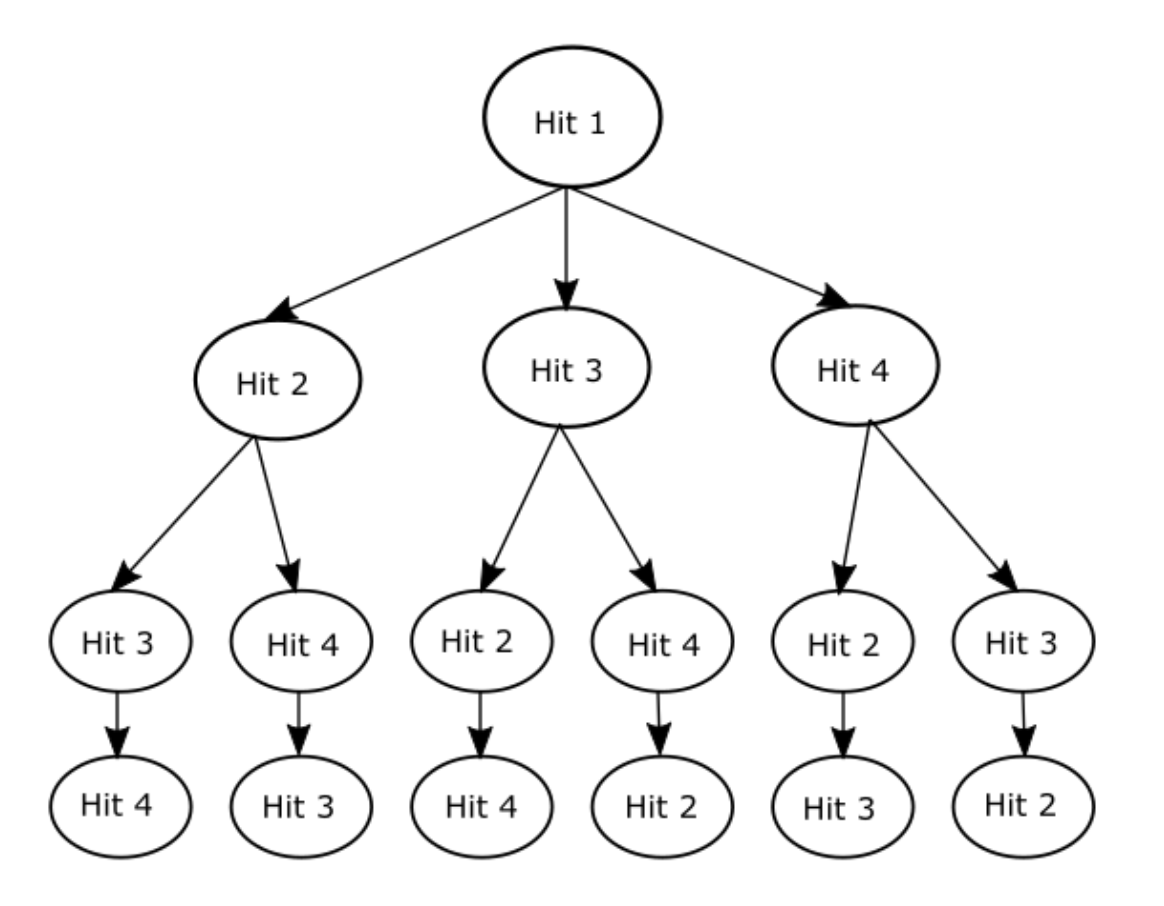
\includegraphics[width=0.6\textwidth]{tree_search_graphic.png}
    \caption{Visual representation of a tree search for one initial hit}
    \label{fig:tree}
\end{figure}

\subsubsection{Recursive algorithm}
In our program, we keep track of the $\chi^2$ value for each \texttt{Hit} we add to the sequence. As we cannot start calculating the $\chi^2$ value without at least one triple, we first take each possible pair of hits and run them through our recursive search algorithm (line \ref{ln:combo}, Algorithm \ref{alg:recon}), keeping a running tally of the $\chi^2$ value and updating it for each child node we process (line \ref{ln:chi2}, Algorithm \ref{alg:recurse}). Theoretically, we could still have to process every possible sequence before reaching the minimum $\chi^2$ value, but, as will be discussed in the following sections, there are ways to prune the tree in order to decrease the average runtime. The real performance improvement of the tree, however, comes from the recursive approach itself. In our iterative approach, we recalculated $\chi^2$ for each node, including those which had the same parent sequence (giving them the same $\chi^2$ value). In the recursive approach, we cut down on these repeat calculations by carrying the $\chi^2$ value through each sequence and only adding onto it when we process a new node. 

\begin{algorithm}
\caption{Tree search reconstruction algorithm for one photon}\label{alg:recon}
\hspace{\algorithmicindent} \textbf{Input:} \texttt{x} - a 1D array of \texttt{Hit} values for one event, \texttt{n} - the number of hits in the event
\begin{algorithmic}[1]
    \State // Pre-compute spatial angles, $\eta$:
    \For {i,j,k in permutations(n, 3)} \label{ln:precompute} \Comment{Loop over all triples}
        \State // Calculate spatial angle:
        \State $\vec{x}_{i}, \vec{x}_j, \vec{x}_{k} \gets$ $x$[i], $x$[j], $x$[k] \Comment{Consecutive hit positions}
        \State $\hat{r}_i, \hat{r}_j \gets |\vec{x}_j - \vec{x}_i|$, $|\vec{x}_k-\vec{x}_j|$ \Comment{Unit vectors along photon direction}
        \State triples[i][j][k] = $\hat{r}_i\cdot\hat{r}_j$ \Comment{Save spatial angle}
    \EndFor
    \State
    \State min$\chi^2 \gets \infty$
    \State $r \gets$ \texttt{NULL} \Comment{\texttt{Result} value}
    \State
    \For {i,j in permutations(n, 2)} \label{ln:combo} \Comment{Loop over all possible pairs of \texttt{Hit} indices}
        \State $\chi^2 \gets$ \texttt{findOptRecursive}(i, j, $n$, 0) \Comment{Pass first two hits to tree search}
        \State
        \If{$\chi^2 <$ min$\chi^2$} \Comment{Check for most likely permutation}
        \State min$\chi^2 \gets \chi^2$
        \State $\eta'_0 = 1 + \frac{1}{W_0}-\frac{1}{W_1} \pm \delta\eta'_0$ \Comment{New $\eta$ value}
        \State r $\gets x[i]$, $x[j]$, $\eta'_0$ \Comment{Update \texttt{Result} with first two hits and $\eta'_0$}
        \EndIf
    \EndFor
\end{algorithmic}
\hspace{\algorithmicindent} \textbf{Output:} r - \texttt{Result} with predicted $\eta$ and first two hit indices
\end{algorithm}

\begin{algorithm}
\caption{Recursive function in tree search}\label{alg:recurse}
\hspace{\algorithmicindent} \textbf{Input:} \texttt{i}, \texttt{j} - current and next hit indices, respectively, \texttt{n} - number of hits left, $\chi^2$ - current $\chi^2$ value for the sequence
\begin{algorithmic}[1]
\Function{findOptRecursive}{i, j, $n$, $\chi^2$}
    \State // Base case:
    \If{n == 0} \label{ln:hitsUsed}
        \State \Return $\chi^2$
    \EndIf
    \State
    \For{each unused \texttt{Hit}, index k}
        \State // Calculate the new energy angle:
        \State $W \gets W - \frac{1}{m_e c^2}E_2$ \Comment{Calculate change in energy}
        \State $\delta W^2 \gets \delta W^2 - \frac{1}{m_e c^2}\delta E_2^2$
        \State
        \State // Calculate $\eta'$ and $\delta \eta'$ \Comment{See Equation \ref{eq:new_compton}}
        \State $\eta \gets$ triples[i][j][k] \Comment{$\delta\eta$ is constant spatial noise}
        \State
        \State Calculate new $\chi^2$ value from $\eta, \eta', \delta\eta, \delta\eta'$ \Comment{See Equation \ref{eq:chi2}} \label{ln:chi2}
        \State
        \State Prune the sub-tree, if possible \Comment{See Section \ref{pruning}}
        \State
        \State \texttt{findOptRecursive}(j, k, $n-1$, new $\chi^2$) \Comment{Move on to next two hits}
    \EndFor
\EndFunction
\end{algorithmic}
\end{algorithm}

\subsection{Pre-calculation of $\eta$ values}
Another performance improvement comes from pre-calculating the spatial angles for each triple, shown in Algorithm \ref{alg:recon} line \ref{ln:precompute}. In the sequential/iterative algorithm (\ref{alg:seq}), we calculate $\eta$ for each triple in each sequence, but, unlike $\eta'$, the spatial angle does not change our calculations based on the sequence it is in. As it is only based on the hits in its given triple, we can calculate $\eta$ only once for each possible triple before we start the tree search and fetch the values when they are needed. This reduces the computation time at each step in photon reconstruction, which greatly increases our reconstruction speed.

\subsection{$\chi^2$ and $\eta$ cutoffs} \label{pruning}

During our tree search, we can \textit{prune} some sub-trees by filtering out certain sequences before we reach the final recursion depth. Depending on the input ordering of hits, we could still end up having to search the whole tree for the correct path, but generally these methods will improve our runtime on average. We can prune a sub-tree if:
\begin{enumerate}
    \item \textbf{The $\chi^2$ value is already greater than the running minimum.}
    
    Since we always assume the sequence with the minimum $\chi^2$ is best, there is no need to check orderings which have already exceeded our best value.
    
    \item \textbf{The cosine of the energetically reconstructed angle, $\eta'$, is greater than 1 by some amount, the $\eta'$ cutoff.}
    
    Our algorithm might return an $\eta'$-value greater than 1 if we either have the wrong ordering of hits or if there is significant noise in the measurement, so we only prune the tree for values significantly above 1, to be safe.
    
    \item \textbf{The $\chi^2$ value of a sequence exceeds what we would expect for the length of the sequence.}
    
    The p-value is related to the probability that the $\chi^2$ we calculate (based on a Gaussian assumption of noise) will naturally exceed a given $\chi^2$ value with the same degrees of freedom. In other words, it is the probability that a good ordering would have a $\chi^2$ value higher than the expected one. We use a look-up table such as the one shown in Figure \ref{fig:p-val} to find the maximum allowed $\chi^2$ value at each step in our calculation and cut off any sequence which exceeds it. The degrees of freedom we use in the $\chi^2$ table is the number of hits in the sequence so far. For example, if we choose a p-value of 0.01, it means we will not accept any orderings that have less than a 1\% chance of being correct. Using this with Figure \ref{fig:p-val}, this means we will prune the tree for any $\chi^2$ value greater than 6.635 after one hit, greater than 9.210 after two hits, greater than 11.345 after three hits, and so on.
    
    \pagebreak
    
    \item \textbf{We have reached some maximum defined recursion depth, which we refer to as the \textit{reconstructed hits}}
    
    Though this is not shown directly in the pseudocode, it is implemented by changing the base case in Line \ref{ln:hitsUsed} of our program to stop the program after a certain number of hits have been processed. We then assume that the sequence with the minimum $\chi^2$ at the cutoff point has the minimum overall $\chi^2$, though there is some chance that this is not the case (the exact probability depends on the cutoff point). This serves to decrease our computation time, but it also means that we do not take all of our data into account, which we expect will decrease our accuracy.
\end{enumerate}

\begin{figure}
    \centering
    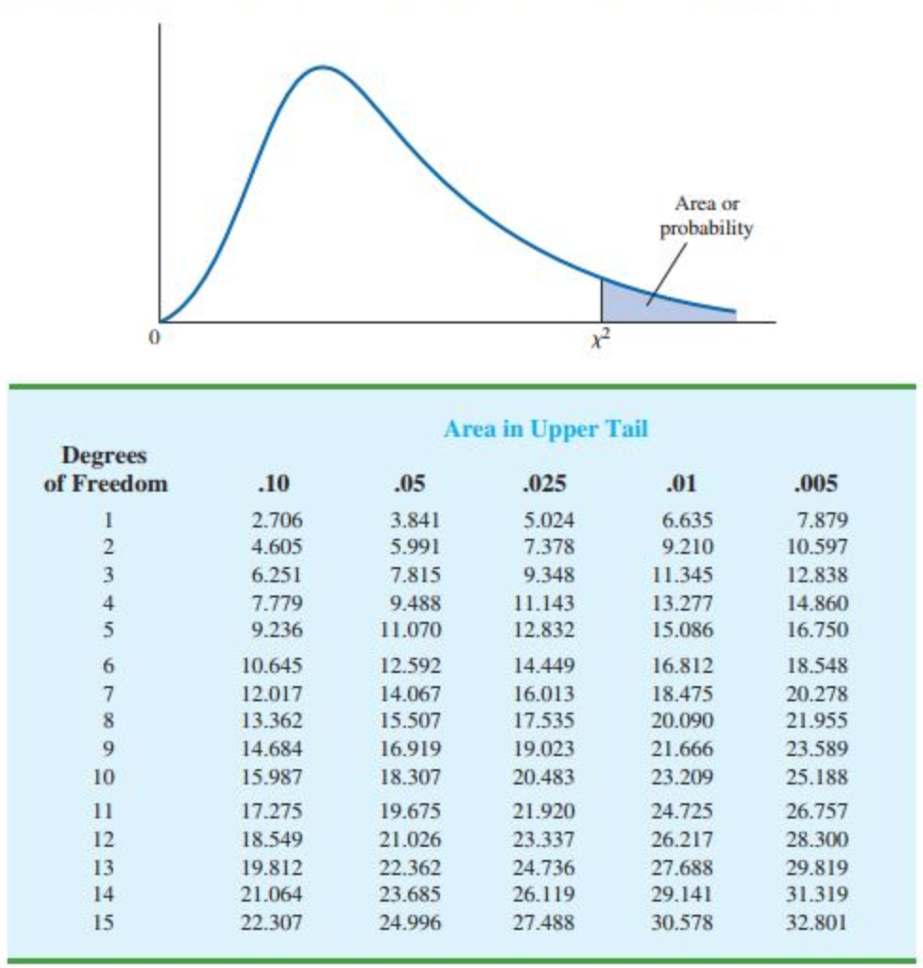
\includegraphics[width=0.5\textwidth]{chi2table.png}
    \caption{An example $\chi^2$ look-up table \cite{chitable}.}
    \label{fig:p-val}
\end{figure}

\section{Parallelism}
Our final performance improvement comes from parallelism. Each photon's computation is independent of the others', so each can be run in a parallel thread to improve the runtime of our algorithm. This also means that if any given photon's computation took longer than expected, there would not be a backlog of events to process which could delay the localization of a gamma-ray burst or other transient. As our current level of parallelism was able to adequately meet our time constraints, we do not seek to increase the reconstruction speed further. However, depending on future time constraints, there are alternate strategies of parallelism and source localization that we could employ to do so.